%==============================================================================
% Voorbeeld gebruik documentklasse hogent-article
%==============================================================================
%
% Compileren in TeXstudio:
%
% - Zorg dat Biber de bibliografie compileert (en niet Biblatex)
%   Options > Configure > Build > Default Bibliography Tool: "txs:///biber"
% - F5 om te compileren en het resultaat te bekijken.
% - Als de bibliografie niet zichtbaar is, probeer dan F5 - F8 - F5
%   Met F8 compileer je de bibliografie apart.
%
% Als je JabRef gebruikt voor het bijhouden van de bibliografie, zorg dan
% dat je in ``biblatex''-modus opslaat: File > Switch to BibLaTeX mode.

\documentclass{hogent-article}

\usepackage{lipsum} % Voor vultekst
\usepackage{float}
\usepackage[belowskip=-10pt,aboveskip=0pt]{caption}

%------------------------------------------------------------------------------
% Metadata over het artikel
%------------------------------------------------------------------------------

%---------- Titel & auteur ----------------------------------------------------

% TODO: geef werktitel van je eigen voorstel op
\PaperTitle{Invloed van diploma en uren wiskunde bij retrieval practice}
% TODO: geef op welk soort artikel dit is
% Dit is typisch de opdracht en het vak waarvoor dit artikel geschreven is, bv.
% ``Verslag onderzoeksproject Onderzoekstechnieken 2018-2019''
\PaperType{Veslag onderzoeksproject Onderzoekstechnieken 2018-2019}

% TODO: vul je eigen naam in als auteur, geef ook je emailadres mee!
\Authors {Robbe Decorte\textsuperscript{1}, Sander Baele\textsuperscript{2}, Niek Gasthuys\textsuperscript{3}, Jurgen De Groote\textsuperscript{4}} % Authors
\CoPromotor{}
\affiliation{\textbf{Contact:}
	\textsuperscript{1} \href{mailto:robbe.decorte@student.hogent.be}{robbe.decorte@student.hogent.be};
	\textsuperscript{2} \href{mailto:sander.baele@student.hogent.be}{sander.baele@student.hogent.be};
	\textsuperscript{3} \href{mailto:niek.gasthuys@student.hogent.be}{niek.gasthuys@student.hogent.be};
	\textsuperscript{4} \href{mailto:jurgen.degroote@student.hogent.be}{jurgen.degroote@student.hogent.be};
}

% TODO: vul de naam van je co-promotor in.
% Als het hier gaat om een voorstel voor de bachelorproef, dan ben je hier
% verplicht de naam van je co-promotor in te vullen. Zoniet, dan kan je het
% leeg laten.
\CoPromotor{}

% Contactinfo: Geef hier de contactgegevens van elke auteur van het artikel (en
% indien van toepassing ook van de co-promotor).


%---------- Abstract ----------------------------------------------------------

\Abstract{Er wordt een experiment uitgevoerd die de learning retention test van 2 verschillende herinneringsmethoden. Een groep studenten neemt deel aan het experiment en zal een tekst meerdere keren lezen en zo beel mogelijk feiten over de tekst verwerken. Na afloop van het experiment testen we onze hypotheses op juistheid en de correctheid van de verkregen resultaten. Om onze hypotheses op te stellen, hebben we gekeken naar volgende variabelen; het aantal uren wiskunde die de student had in het middelbaar, de secundaire afstudeerrichting, het hebben van ouders met universitaire achtergrond en de interessie bij het maken van de opdracht van de student. Bij het toetsen van deze hypotheses zagen we dat er moeilijk een verklaarbare link gelegd kan worden tussen enkele bovenstaande variabelen.
}

%---------- Onderzoeksdomein en sleutelwoorden --------------------------------
% TODO: Vul de sleutelwoorden aan.


\Keywords{Learning; Retention; Retrieval; Practice;}
\newcommand{\keywordname}{Sleutelwoorden} % Defines the keywords heading name

%---------- Titel, inhoud -----------------------------------------------------

\begin{document}
	
	\flushbottom % Makes all text pages the same height
	\maketitle % Print the title and abstract box
	\tableofcontents % Print the contents section
	\thispagestyle{empty} % Removes page numbering from the first page
	
	%------------------------------------------------------------------------------
	% Hoofdtekst
	%------------------------------------------------------------------------------
	
	\section{Inleiding}
	
	Het achteruit gaan van het geheugen is een fenomeen waar vroeg of laat iedereen last van heeft, de mate is deels te wijten aan beslissingen van de persoon zelf, maar dit kan plots gebeuren door ziekte, ongeval ... In dit onderzoek gaan we op zoek naar data die kan bevestigen dat je door middel van gedachten te linken je meer kan onthouden zonder rekening te houden met problemen aan het geheugen. Het geheugen is een zeer actueel onderwerp en daarom kan deze studie makkelijk gelinkt worden aan onderzoekstechnieken die we overnemen van studies die zich reeds hebben bewezen. Om een steekproef te bekomen die groot genoeg is en representatief is tegenover de gemeenschap richt deze studie zich op 2e jaars studenten toegepaste informatica, die het vak 'onderzoekstechnieken' volgend aan HoGent. De leerlingen komen stuk voor stuk uit een verschillende achtergrond en zorgt dus voor genoeg variatie tussen de testpersonen.
	
	\section{Overzicht literatuur}
	
	\subsection{Robbe Decorte - Literatuur}
	Evaluating storage, retention, and retrieval in disordered memory and learning \autocite{BuschkeFuld1974}
	
	Ze bespreken 2 simpele manieren om bij verschillende mensen het geheugen te quoteren en met
	elkaar te vergelijken (nl. selectief herinneren en restrictief herinneren)
	Bij selectief herinneren herhalen ze enkel de woorden die je niet genoemd hebt in de test die direct volgt na het
	opzeggen van alle woorden tot je 2 opeenvolgende testen alle woorden kan opzeggen, restrictief gaat doortot je elk woord minstens
	1x kan herinneren zodat de lijst inkrimpt (elk woord wordt na het herinneren ervan uit de lijst gehaald).
	Woorden die je kan herinneren in een sessie waar die voorgaand niet in gezegd is, komen uit je lange
	termijn geheugen. Het falen van de patiënt kunnen we linken aan het niet (snel genoeg) kunnen onthouden van woorden in het
	lange termijn geheugen. We kunnen zeggen dat een lijst gekend is als de patiënt consistent alle woorden kan herhalen, het heeft dus geen nut als
	je uit het lange termijn geheugen woorden kan onthouden wanneer je andere woorden die net gezegd zijn niet kan herhalen.
	Deze methoden zijn enkel nuttig om abnormaliteiten vast te stellen (in dit geval alcoholisme) maar vertellen weinig over de staat van het geheugen
	als je 2 patiënten met hetzelfde probleem met elkaar vergelijkt. De patiënt had bij beide methoden 6 pogingen nodig vooraleer die in staat was om alle woorden
	op te zeggen, maar was niet in staat om deze te herhalen in de volgende sessie van selectief herinneren. De beste manier om dit aan te pakken is door je visie te 
	veranderen, je mag het niet zien als 10 individuele woorden maar als een lijst waar je zelf een link moet leggen tussen verschillende woorden. Op deze manier kunnen wij
	een hypothese opstellen, "Door een link te leggen tussen de woorden zorg je niet alleen dat je in de volgende sessie een hoger aantal woorden kan herhalen maar ook 
	dat je na enkele uren meer woorden kan opsommen dan iemand die deze manier niet toepast". Deze hypothese lijkt me belangrijk voor het resultaat maar is niet behandeld in deze studie.
	
	
	Preserved learning and retention of pattern-analyzing skill in amnesia: dissociation of knowing how an knowing that \autocite{CohenSquire1980}
	
	Er wordt onderzocht in hoeverre een persoon verschillende soorten informatie kan onthouden terwijl hij aan geheugenverlies lijdt, de 2 soorten informatie die ze hier onderscheiden zijn
	handelingen waarvan je weet hoe ze werken (data based) en informatie waarvan je weet dat het iets doet, zoals bijvoorbeeld de naam van een persoon (hier is geen logica aan verbonden).
	De hypothese stelt dat geheugenverlies minder effect heeft op de 1e soort dan initeel gedacht. Ze onderzoeken dit door mensen met een sterke vorm van geheugenverlies enkele zaken laten
	uitvoeren, dit telkens iets fysiek (nl. traceren en spiegelen). Je ziet in de resultaten dat dit elke poging verbeterde terwijl de patiënt zich niet / amper kon herinneren dat hij deze 
	handelingen eerder had uitgevoerd. In een 2e experiment laten ze de patiënten 3 maanden lang met 3 sessies per dag lezen, door deze skill te trainen verliezen ze niet het vermogen om te
	lezen terwijl dit bij een normaal geval wel het geval is. Deze mensen kunnen hun geheugen dus trainen op motor skills zonder dat ze deze onthouden, ze linken dit aan een invloed van het
	zenuwstelsel waar enkele simpele handelingen een soort van genaturaliseerd worden. De data die hier is gevonden geeft ons niet enkel een beter beeld van de ziekte zelf maar zou moeten
	helpen bij het opzetten van AI en het bekijken van cognitieve wetenschappen binnen de computerwereld, er zijn namelijk al jaren discussies over hoe ze dat fenomeen moeten beschrijven.
	
	\subsection{Sander Baele - Literatuur}
	Team-based learning enhances long-term retention and critical thinking in an undergraduate microbial physiology course \autocite{Mcinerney2003}
	
	Team-based learning vereist een speciale aanpak. Het vereist dat het vak geherstructureerd word om nieuw gevormde groepen en teams uit de dagen met complexe, uitdagende, leerrijke taken. Er zijn algemeen gezien 3 aanpakken die zich goed van elkaar onderscheiden, namelijk: coöperatief leren, probleem-gebaseerd leren, en team-gebaseerd leren.
	Coöperatief leren vereist weinig herstructurering aan het opleidingsonderdeel. Er worden groepen gevormd om een bestaand onderdeel uit het opleidingsonderdeel te volbrengen.
	Probleem-gebaseerd leren vereist een grotere herstructurering van het opleidingsonderdeel. Het probleem komt er, nog voordat alle relevante materie gezien is. Deze aanpak bevindt zich tussen coöperatief leren en team-gebaseerd leren.
	Team-gebaseerd leren is op zich gelijkaarde aan probleem-gebaseerd leren, maar studenten vergaren eerst de nodige leerstof. Dit gebeurd voor men begint aan het probleem. Er worden geen rollen verdeeld, en tussenkomst van een leerkracht is optioneel.
	De eerste fase van de 3, is de opzet fase. Tijdens deze fase vergaren de studenten de introductie informatie van lesmomenten, lezingen, enz. en worden ze getest op deze informatie. Men wordt individueel getest. Erna maken ze direct dezelfde test in groep. Beide testen worden gescoord en tellen mee voor de uiteindelijke scores. Hierop volgt nog feedback van de leerkracht indien nodig.
	De volgende fase is de toepas fase. De teams krijgen toenemend uitdagende projecten, dit zijn louter oefeningen, en tellen niet mee voor de score voor het vak. De leerkracht gaat met de studenten in gesprek over hun conclusies, en vergaart zo feedback over de kwaliteit van de antwoorden. 
	De derde en laatste fase is de scorings fase. Deze fase zal bijdragen van 20 tot 40 procent van de score die de student krijgt voor het vak. Uiteraard volgt er ook een peer evaluation, waarin de studenten elkaar kunnen beoordelen op basis van elkanders bijdrage.
	De kwaliteit van de projecten was het eerste criterium die belangrijk was om de educatieve waarde te bepalen van dat project. Deze waarde bepalen omvatte meerdere pijlers, zoals het detail van analyse, de hoeveelheid materie uit het opleidingsonderdeel, de integratie van materie uit andere vakken, en creatieve en intuïtieve deducties die teams zelf maakten.
	De finale testen werden zodanig opgesteld dat ze qua formaat, uitgebreidheid, en moeilijkheidsgraad, gelijk waren tussen jaren mét en jaren zonder groeps-gebaseerd leren.
	Er werden 2 vragen gesteld in jaren mét en jaren zonder groeps-gebaseerd leren. Namelijk de hoeveelheid informatie de student zelf vond dat hij/ zij opgenomen had, en de score die hij/ zij gaf aan de leerkracht met betrekking tot de mate waarin die leerkracht kritisch denken promootte.
	Er werd Chi-square analyse gebruikt om de significantie hiervan te bepalen; die was 0.05.
	Men begon het eerste jaar (2000) met toevoeging van quizzen. Deze zorgden voor een positieverer attitude, maar qua scores presteerden de studenten nog vrij laag. Het was pas dankzij de team-gebaseerde projecten dat deze omhoog gingen.
	In het jaar 2001 en 2001 gebruikte men de projecten. Men zag dat evenveel studenten boven de 90 procent zaten als de jaren voordien. Aan de hand van Chi-square analyse kon men dus aantonen dat de moeilijkheidsgraad dezelfde was gebleven. Het aantal studenten die tussen 70 procent en 90 procent score, steeg wel aanzienlijk. Meer dan 80 procent van de studenten was positief ten opzichte van het opleidingsonderdeel, de docent, en de team activiteiten.
	Men kan wel degelijk vaststellen dat team-gebaseerd leren voordelen heeft bij het verwerken van grote hoeveelheden informatie. We moeten wel meegeven dat dit zo blijkt bij een opleidingsonderdeel microbiologie. Dit kan natuurlijk anders zijn bij andere soorten materie.
	
	Memory vocabulary learning strategies and long-term retention \autocite{Nemati2009}
	
	Volgens een studie van \autocite{Nielson2006}, is het beter om in de vroegere stadia van het aanleren van een taal, 'de-contextualized' woorden aan te leren. Hij toont aan dat dit beter is om een stevige basis te leggen. Naarmate men vordert in de taal, zou men gelijdelijk aan over moeten gaan naar 'contextualized' leren. Een hypothese van \autocite{CraikTulving1975} suggereert dat het niet belangrijk is hoe recent woorden geleerd zijn, maar hoe diep men het woord in zich neemt. Dit betekent, hoe meer de persoon in kwestie het woord manipuleert, en cognitief opneemt, hoe beter het behoud ervan. In deze studie zijn de geheugen strategieën onze grootste focus, opgedeeld in 4 sets. Deze sets zijn ``aanmaken van mentale linken'', ``toepassen van beeld en geluid'', ``goed hernemen'', en ``gebruik maken van acties''. Deze klassen werden opgedeeld door \autocite{Oxford1990}. We gaan ons nog meer bezighouden met drie substrategieën: groeperen, acroniemen maken, en beelvorming. Het groeperen verwijst naar het klasseren van taal in betekenisvolle contexten, om het zo makkelijker te maken om te herinneren. Acroniemen gebruiken is volgens Oxford nieuwe woorden in een context zetten, om ze beter te herinneren. Als laatste kunnen we ook beeldvorming gebruiken om opnemen van nieuwe woorden te faciliteren.
	Enkele onderzoeksvragen die we gesteld hebben zijn de volgende:
	Is er een verschil tussen de prestaties van de leerling in elke sub-strategie en de strategie die de leerling volgens zichzelf gebruikt?
	Is er een impact van aanleren van sub-strategies aan leerlingen ten opzichte van de control groups?
	De proefpersonen van deze studie zijn 310 vrouwelijke studenten, die nog niet aan hoger onderwijs doen. Het onderzoek werd in India uitgevoerd. De moedertaal daar, is Kannada. Deze taal werd gebruikt om de studenten Engels aan te leren. De studenten waren tussen 16 en 18 jaar. Uiteindelijk ware ner 140 studenten in de control group, en 170 in de experimentele groep.
	Om data te verzamelen werd aan de studenten gevraagd een vragenlijst in te vullen en aan te geven hoeveel ze sommige strategieën denken gebruikt te hebben.
	Er werd ook gebruikt gemaakt van een Vocabulary Knowledge Scale (VKS). Dit om een idee te krijgen van de vooruitgang in kennis.
	De studie verliep in 3 stappen: De eerste stap is de pre-test. 
	Dit is de eerder vermelde zelf-evaluatie vragenlijst en de VKS. 
	Bij deze pre-test horen ook nog de lessen.
	Lessen in de control group gebruikte verschillende methoden, zoals de presentatie van individuele woorden, orale uitspraak, de woorden op het bord schrijven, een kleine beschrijving ervan, synoniemen en antoniemen aanhalen, en minimale contexten (zoals een kleine zin met het woord in).
	In de experimentele groep begon men met de student kennis te laten maken met strategieën, en zo een strategy awareness te creëren. Bij de eerste strategie (groeperen), moesten de studenten woorden bij hetzelfde thema plaatsen. Bij de tweede strategie, moesten de studenten voor woorden een afkorting maken, om zo de woorden beter te onthouden. Bij de derde strategie, moesten de studenten het visueel voorstellen.
	De tweede stap van het onderzoek, is de post-test 1. Na een lesmoment wordt een korte termijn test gegeven.
	De derde stap van het onderozke, is de post-test 2. Na 2 weken werd er weer een test gegeven op de kennis.
	De eerste onderzoeksvraag was de vraag waarbij studenten zelf moesten evalueren hoezeer ze de strategieën gebruikten. Er bleek dat de control groups overschatten hoeveel ze de strategiën gebruikten. Uiteindelijk deden de experimentele groepen het iets beter dan de control groups. En na de twee weken gingen de scores van de experimentele groepen ook minder achteruit.
	Ook is het duidelijk dat er wel degelijk een impact is van het aanleren van de strategieën aan de leerlingen
	We concluderen dat het toepassen van deze strategieën het opnemen van nieuwe woorden beïnvloed op een positieve manier. Deze diepere manier van aanpakken, en aanleren op een efficiëntere manier, heeft positieve gevolgen voor het behoud van de opgedane kennis.
	
	\subsection{Niek Gasthuys - Literatuur}
	
	Physical Exercise Performed Four Hours after Learning Improves Memory Retention and Increases Hippocampal Pattern Similarity during Retrieval \autocite{Drongen2016}
	
	In dit artikel gaat men na of dat fysieke inspanningen zoals sporten het lange termijngeheugen positief beïnvloed of niet. Hiervoor heeft men 72 willekeurige mensen opgedeeld in 3 groepen. Ze leren allemaal een lijst van foto’s gerelateerd met een plaats onder exact dezelfde omstandigheden. Het enige verschil tussen de groepen is wanneer men een fysieke inspanning doet na het leren van de foto’s. De eerste groep doet geen inspanning, de tweede na 4 uur van het leren en de derde direct na het leren. Uit het experiment bleek dat de groep die na 4 uur een fysieke inspanning deed de beste resultaten had en dus de meeste foto’s kon oproepen 48 uur na het instuderen. Uit dit experiment kunnen we dus de conclusie trekken dat een goed getimede fysieke inspanninng een positieve invloed heeft op het lange termijngeheugen. We kunnen dit perfect testen tijdens ons eigen onderzoek door 2 groepen te vormen die een reeks van woorden instudeert en 1 van de 2 groepn gaat nadien een fysieke inspanning doen. Hetgeen nog onbreekt in dit onderzoek uit het artikel is de manier waarop we te weten kunnen komen welk moment ideaal is om de beste invloed te hebben op het lange termijngeheugen zodat we met een manier kunnen komen die veel efficienter kan toegepast worden tijdens het studeren. We kunnen dit doen door het experiment een aantal keer te herhalen en dan te kijken welke factor steeds overeenkomt met de beste testresultaten en zo de tijd te kunnen bepalen. Op deze manier gaan we het onderzoek verder aanscherpen.
	
	Repeated retrieval during learning is the key to long-term retention \autocite{Karpicke2007}
	
	In dit artikel doet men 2 experimenten. In het eerste experiment gaat men 60 studenten opdelen in drie groepen. Elke groep voert een ander soort studiemethode uit. De eerste groep voert de stadaard methode uit, namelijk eerst een studietrial, dan een testtrial enzovoort. De tweede groep voert de repeated study methode uit(SSST), namelijk 3 keer studeren en 1 keer testen en de laatste groep voert de repeated test methode uit(STTT), namelijk 3 maal testen na 1 keer leren. Na het experiment gaan we zien welke groep de meeste woorden kan oproepen uit zijn langetermijngeheugen van een lijst van woorden. Uit het experiment bleek de eerste groep die studeren en testen heeft afgewisseld de meeste woorden te kunnen oproepen. In het tweede experiment gaan we na of er invloed is wanneer we testen en leren constant wisselen of dat we bijvoorbeeld eerst 2 leerfasen doorlopen en dan 2 testfasen. Uit het tweede experiment bleek de STSnT conditie de beste methode te zijn. Dit is de methode waar men de woorden tijdens afwisselende trials heroproept en studeert. Dus met andere woorden dat we de lijst altijd heroproepen per keer dat we een testfase of leerfase doorlopen en de woorden die we al kennen ook nog steeds oproepen. Deze manier bleek uit het tweede experiment wel 100 procent keer beter te zijn voor het lange termijngeheugen dan dat we de woorden die we al kennen niet meer herhalen in toekomstige leer of studeerfasen.We kunnen dit tijdens ons onderzoek niet echt veel meer aanscherpen omdat de 2 experimenten de mogelijke twijfelgevallen uitsluit. Het artikel zijn experimenten zijn zo goed als waterdicht. Hetgeen we wel kunnen doen is het eerste artikel over de invloed van fysieke inspanningen op lange termijngeheugen combineren met de methode uit dit artikel en kijken of dit nog een beter resultaat heeft of niet. En zo kunnen we dit onderzoek toch nog aanscherpen.
	
	
	\subsection{Jurgen De Groote - Literatuur}
	
	The impact on retention of interventions to support distance learning students \autocite{Simpson2004}
	
	Dit artikel bespreekt hoe leerlingen falen in hun richting en wat eraan kan gedaan worden. Hieruit kan worden afgeleid dat de interactie met de leerkracht in de les een grote invloed heeft op slaagkansen. Op eerste zicht heeft dit niet veel te maken met de effectiviteit van studiemethodes, maar dit artikel bespreekt ook hoe studenten die deze interactie niet hebben het veel moeilijker hebben in hun studierichting. In ons geval gaan studenten die afstandsonderwijs volgen dus moeilijker slagen. De aanwezigheid in de lessen gaat dus ook je studiemethode beïnvloeden. Het volgen van lessen is namelijk één van de belangrijkste studiemethoden om alles voor een eerste keer wat in te studeren. Mensen die alles voor het eerst moeten leren gaan een andere studiemethode moeten hanteren dan mensen die wel naar de lessen gingen. Voor hen gaat alles veel vlotter verlopen. In ons onderzoek gaan we dit uiteraard niet kunnen testen. Hiervoor zouden we een groep leerstof voor het eerst moeten laten studeren en een andere groep die de leerstof studeert nadat het door een leerkracht interactief werd uitgelegd. De conclusie uit dit artikel is dat het extreem belangrijk is lessen te volgen voordat je gaat studeren. Hier bovenop help een interactieve les ook hopen meer dan een niet interactieve les.
	
	Comparative effects of test-enhanced learning and self-explanation on long-term retention \autocite{LarsenButlerRoediger2013}
	
	Dit artikel heeft onderzoek gedaan om de self-explanation studiemethode te vergelijken met repeated testing. Voor dit onderzoek heeft men 47 studenten willekeurig opgedeeld in 4 groepen. Eén groep ging regelmatig testen met gebruik van self-explanation. De tweede groep ging regelmatig testen afleggen zonder self-explanation. De derde groep ging normaal studeren met self-explanation. En ten slotte de laatste groep ging normaal studeren zonder self-explanation. Na 6 maanden werd er bij iedereen dezelfde test afgenomen. Uit dit onderzoek werd duidelijk dat self-explanation een goede invloed had op de resultaten van de studenten. Studenten die de leerstof zichzelf uitlegde tijdens het studeren krijgen betere resultaten dan degenen die dit niet deden. Hiernaast haalden de studenten die regelmatig een test deden veel betere resultaten dan de studenten die dit niet deden. Als we deze twee methodes dus vergelijken kunnen we duidelijk zien dat beide een goede invloed hebben, maar het regelmatig testen effectiever is dan self-explanation. Uiteraard is de beste optie een combinatie van beiden. De studenten die regelmatig testen ging afleggen met self-explanation behaalden dan ook de beste scores van allemaal. In onze eigen onderzoek kunnen we het regelmatig testen zelf niet uitproberen aangezien we op korte termijn gaan moeten leerstof studeren en een test afnemen. Wat we wel gelijkaardig kunnen onderzoeken is de invloed van self-expanation. We kunnen 2 groepen maken waar eentje tijdens het studeren tegen zichzelf alles gaat uitleggen en de andere die dit niet doet. Zo kunnen we vergelijken of onze resultaten overeenkomen met de studie die in dit artikel werd uitgevoerd.
	
	
	\section{Methodologie}
	
	De studenten worden lukraak in 2 gelijke groepen verdeeld (respectievelijk groep A en groep B) waarbij in elke groep nog een onderscheid gemaakt wordt tussen studenten die naar muziek luisteren en studenten die niet naar muziek luisteren, we verkrijgen dus een 4 verschillende onderschijdingen. Beide groepen analyseren een tekst die gevuld is met weetjes over Charles Darwin en trachten zo veel mogelijk informatie in hun geheugen op te nemen. Groep A, die retrieval practice toepast, zal na de 1e leesronde zo veel mogelijk weetjes neerschrijven terwijl groep B een oefening maakt die hun gedachten moet afleiden van de tekst. 5 minuten later wordt de tekst opniew gelezen en wordt het proces nogmaals herhaald. Bij het 2x lezen van de tekst krijgt elke groep een officieel invulblad waarmee een score kan toegekend worden. De eerstvolgende week wordt deze test nogmaals uitgevoerd waardoor we voor (bijna) elk persoon 2 scores hebben. 
	Vooraleer het experiment begint stellen we een aantal hypotheses op aangevuld met een nulhypothese en vullen we deze aan met grafieken en andere toepasbare statistische testen. Eenmaal we over de resultaten beschikken, zullen we deze toetsen vergelijken met de bekomen data.
	Algemeen zullen we in deze studie eerst kijken of we een verschil zien in de resultaten bij studenten die Retrieval Practice toepasten en degene die dit niet deden. We zullen dit doen door een data-analyse in het programma R. Daarnaast kiezen we verder ook nog variabelen die mogelijks de resultaten zullen beïnvloeden en maken we ook hier grafieken van.
	
	\section{Verwachte resultaten}
	\label{sec:verwachte_resultaten}
	We verwachten dat de studenten die Retrieval Practice toepasten, beter zullen scoren op de test en duidelijker beter zullen scoren op de test de week nadien. De groepen die naar muziek luisterden, zullen iets minder scoren dan de groepen die dit niet deden. Als variabelen van deze studie hebben we ons vooral gebaseerd op de achtergrond en ervaring van de student. We kijken naar de achtergrond van de ouders, die van de student, en zijn eerdere studierichtingen. Deze pijlers hangen goed samen omdat ze een beeld geven over de situatie van de student.
	
	\begin{figure}[H]
	 	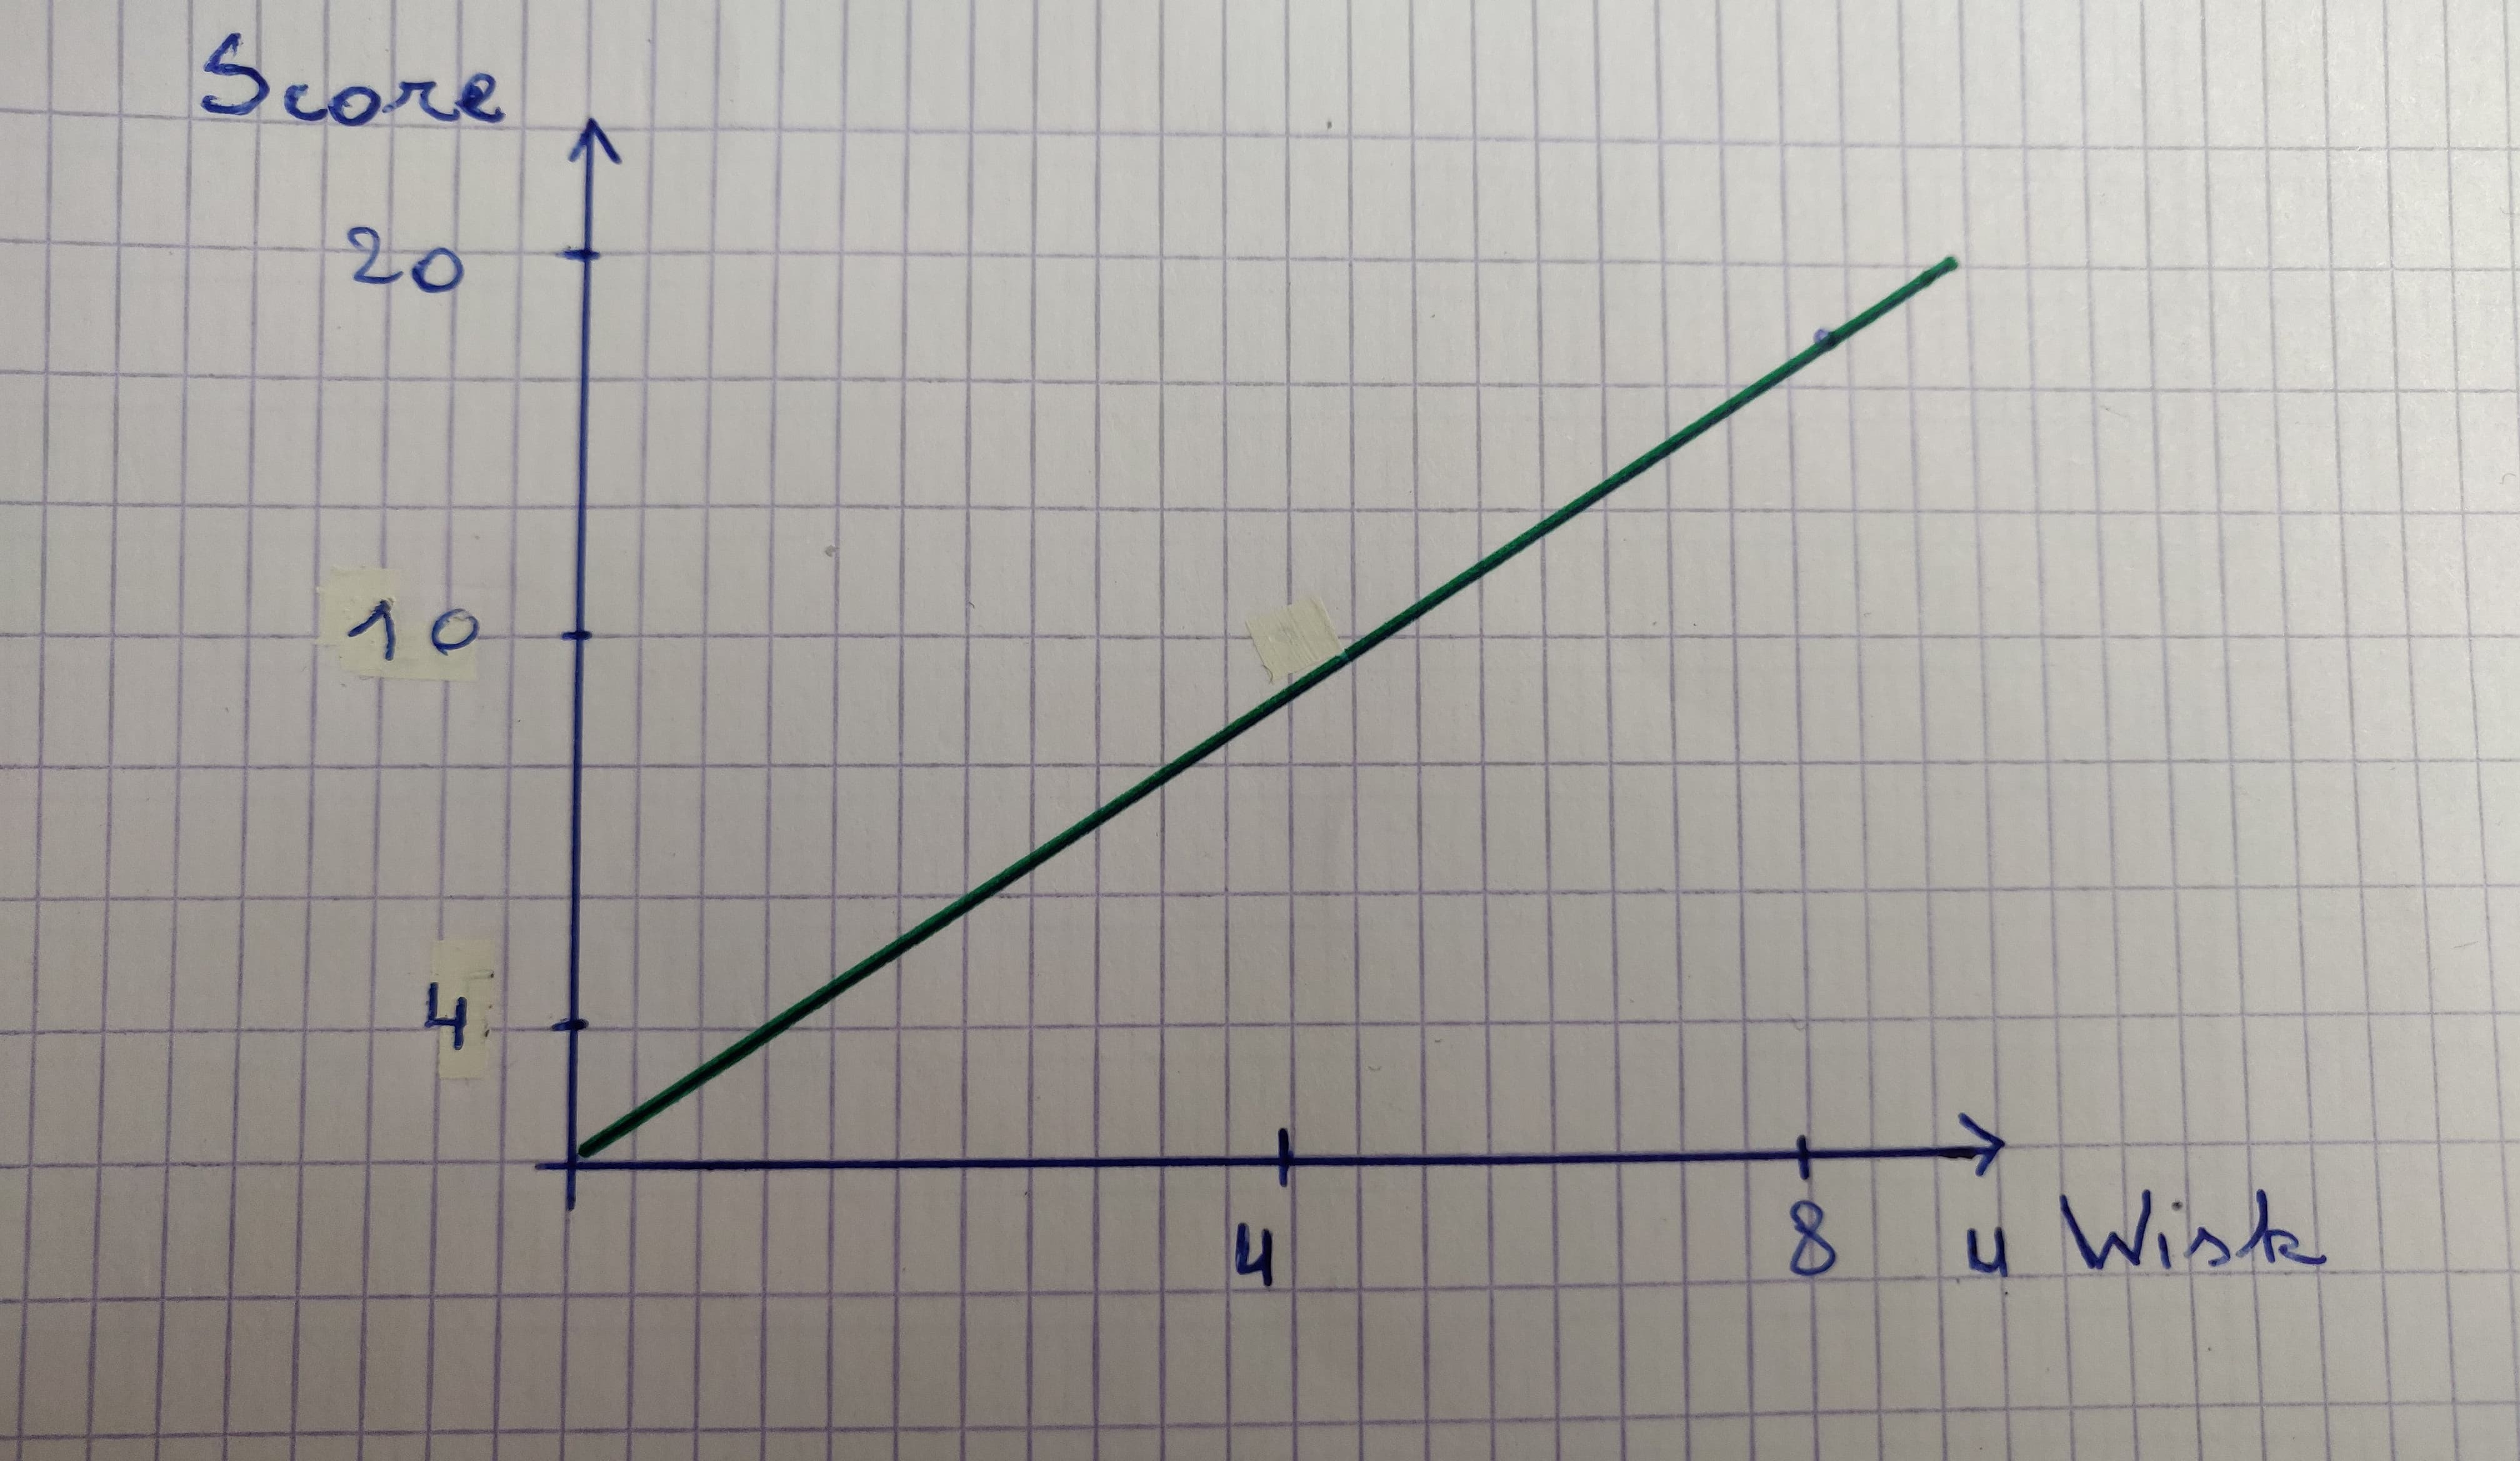
\includegraphics[width=\linewidth]{img/imgg1.jpg}
 		\caption{Mockgrafiek \textbf{$H_1$}, invloed van het aantal uren wiskunde op de score}
	\end{figure}
	 
	\textbf{$H_0$}: Het behaalde diploma heeft geen invloed op de score
	
	\textbf{$H_1$}: Studenten met een hoog aantal uren wiskunde in het secundair onderwijs scoren beter dan die met een laag aantal uren wiskunde (minder dan 4 uur).
	
	\textbf{$H_2$}: Studenten met minstens één ouder die een universitair diploma bezit, hoger zullen scoren dan studenten die ouders hebben zonder universitair diploma.

	\textbf{$H_3$}: Studenten met een algemenere secundaire achtergrond (ASO) beter scoren dan degene die iets anders deden.
	\begin{figure}[H]
		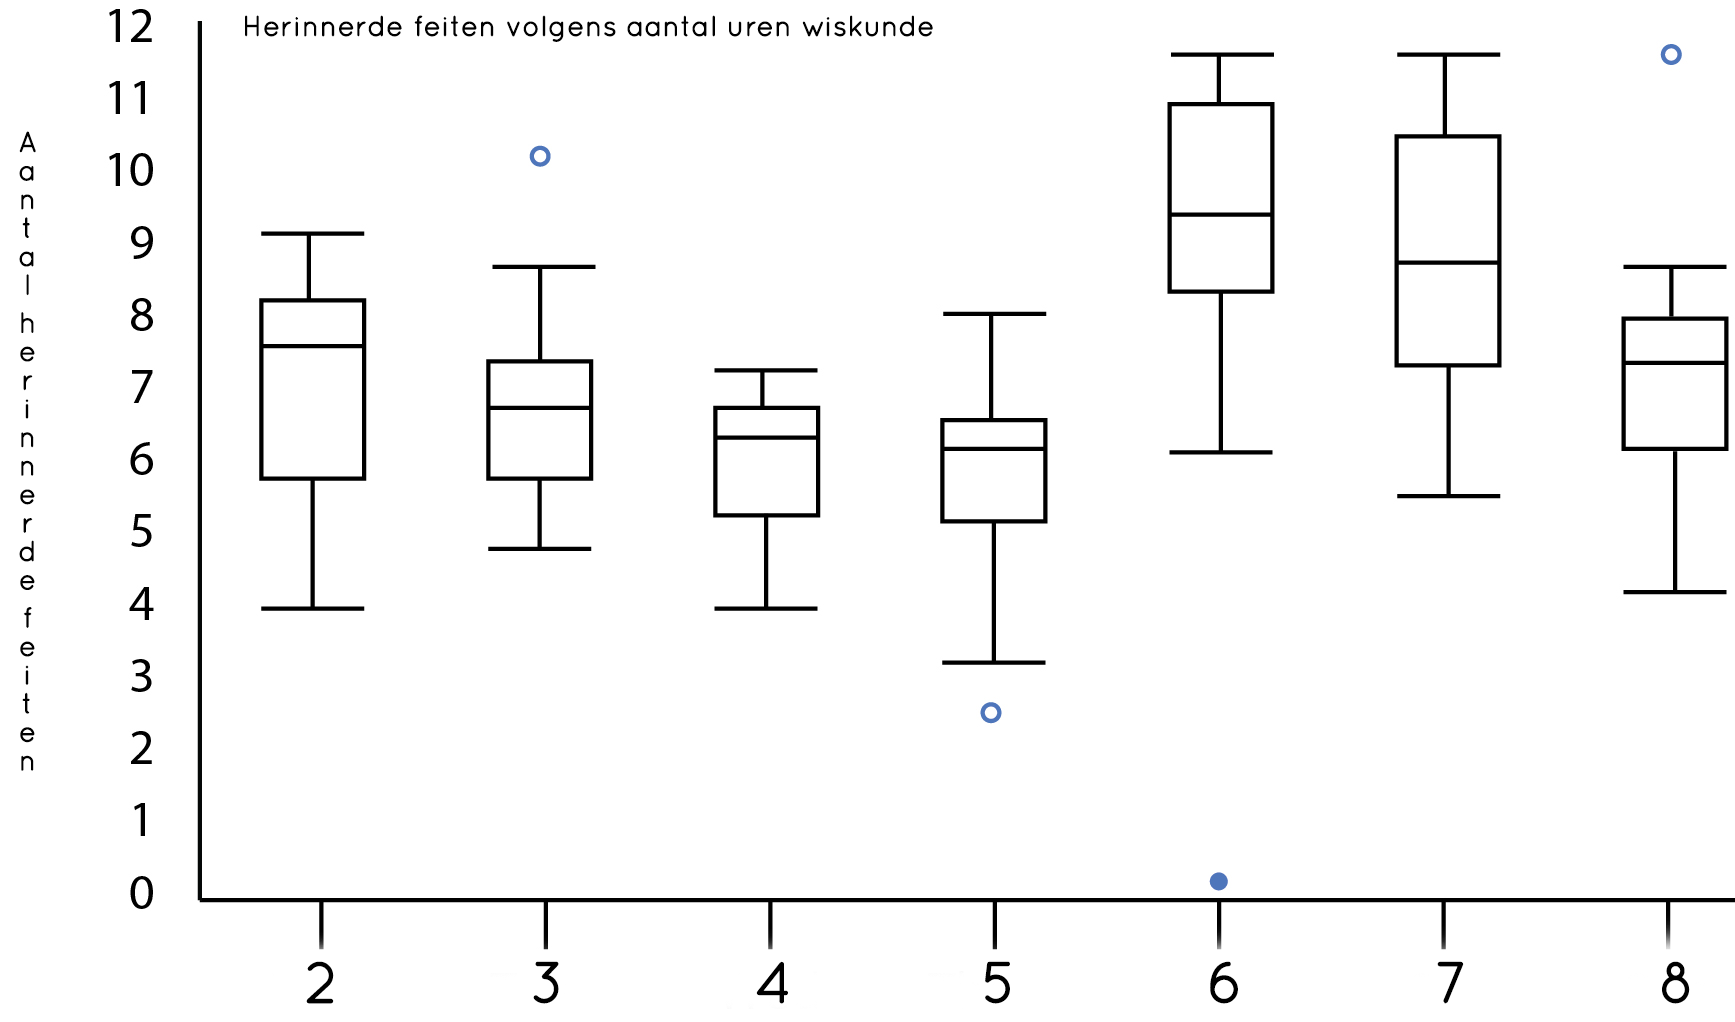
\includegraphics[width=\linewidth]{img/mockboxplot.png}
		\caption{Mockgrafiek \textbf{$H_2$}}
	\end{figure}
	\begin{figure}[H]
		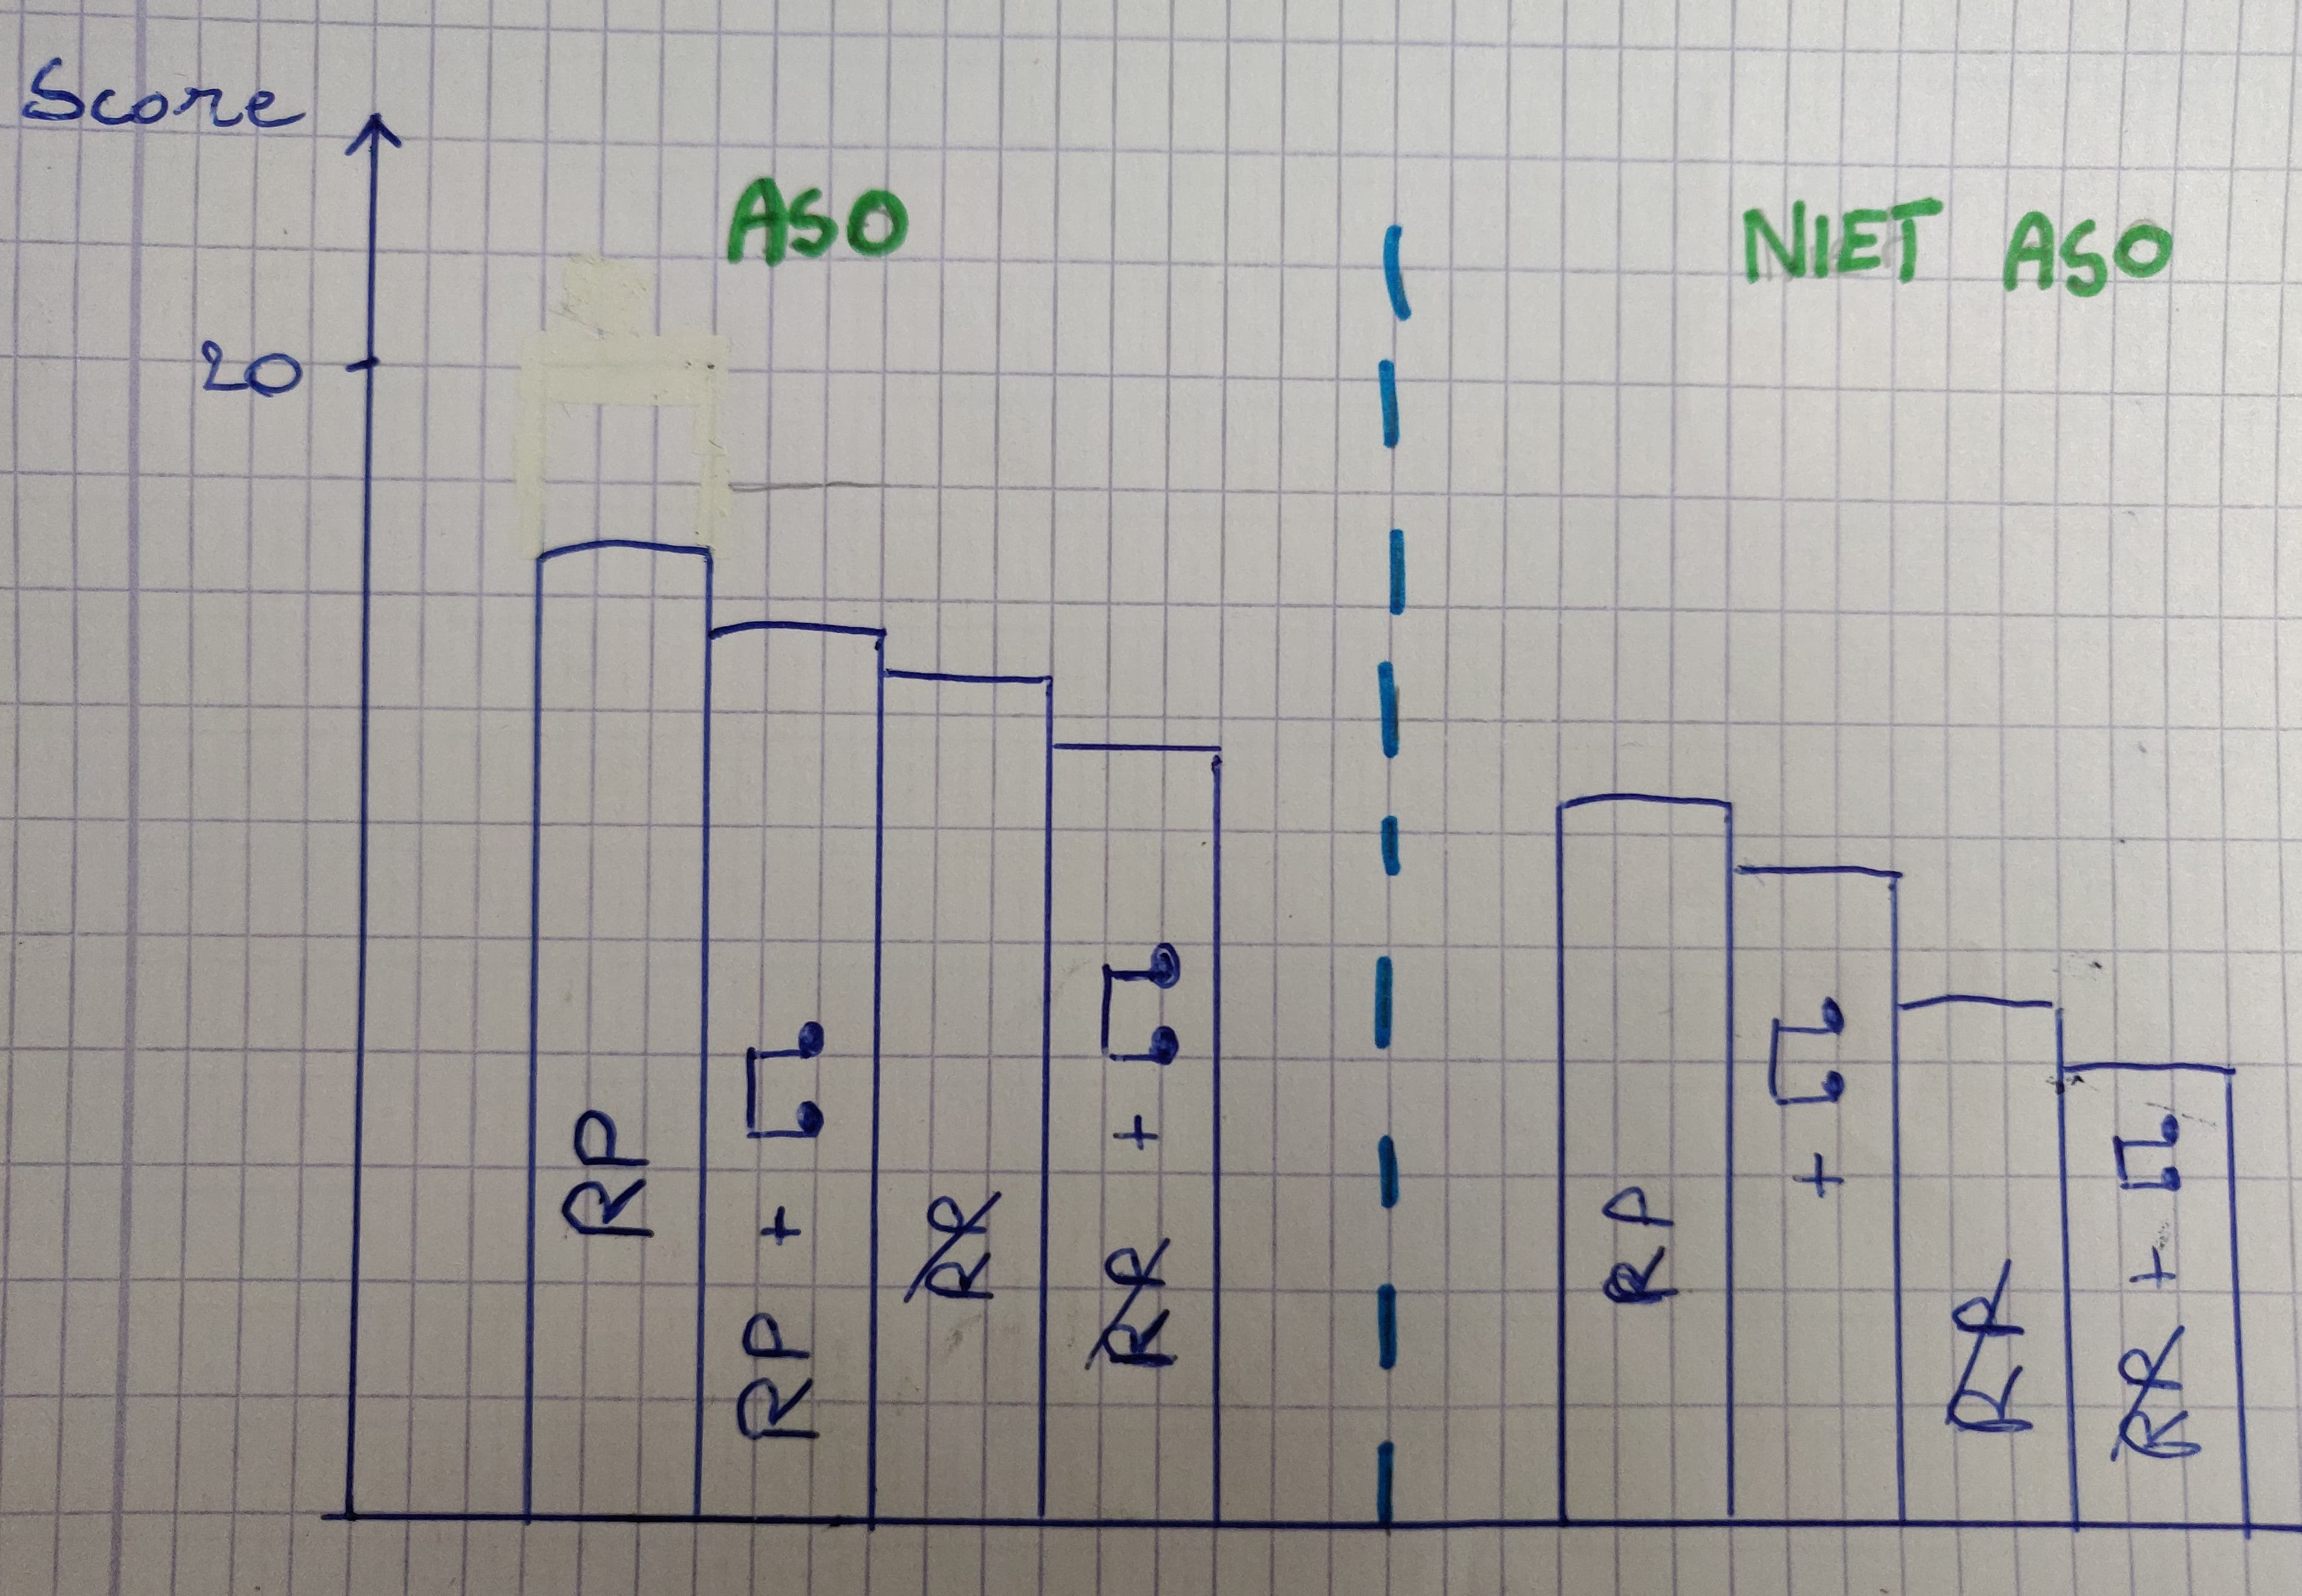
\includegraphics[width=\linewidth]{img/imgg2.jpg}
		\caption{Mockgrafiek \textbf{$H_3$}}
	\end{figure}
	
	%---------- experimenten ----------------------------------------------
	\section{Experimenten}
	Tijdens 2 oefensessies krijgen de leerlingen een artikel. In dit geval bestaan de werkgroepen uit 4 personen die je verder kan verdelen in 2 volgens de vermelding in Methodologie. Beide groepen bestuderen eerst het 
	artikel waarna Groep A de tekst nog eens leest en Groep B een leeg blad krijgt en zoveel mogelijk weetjes uit de tekst moet neerschrijven. Dit proces herhalen we nog een 2e keer waarna iedereen een officieel antwoordenblad krijgt waar hij/zij hun definitieve antwoorden moet opschrijven. Hetzelfde experiment wordt de week erna nog eens indentiek uitgevoerd waardoor we 2 verschillende scores per persoon krijgen.
	De testen worden niet streng verbeterd, het gaan namelijk over de algemene feiten die je moet herinneren en het volstaat dus om 'Darwin-dag' te herinneren in de plaats van de volledige datum terwijl deze ook in de tekst vermeld is. Algemeen zullen we ook bekijken of de Retrieval Practice al dan niet een impact had op het herinneren van de inhoud op de dag zelf en een week nadien.
	
	
	\section{Analyse resultaten}
	 Als we algemeen kijken, dus nog niet naar de variabelen, dan zien we al enkele resultaten. Hoewel we verwachtten dat RP gemiddeld altijd meer zou scoren dan de de tegenpartij, is dit enkel zo bij de groepen die muziek luisterden. Bij de groepen die geen muziek luisterden scoren de groepen die geen RP gebruikten meer dan degene die het wel gebruikten. Het beluisteren van klassieke muziek heeft dus wel degelijk een invloed op het geheugen.
	
	\begin{figure}[H]
		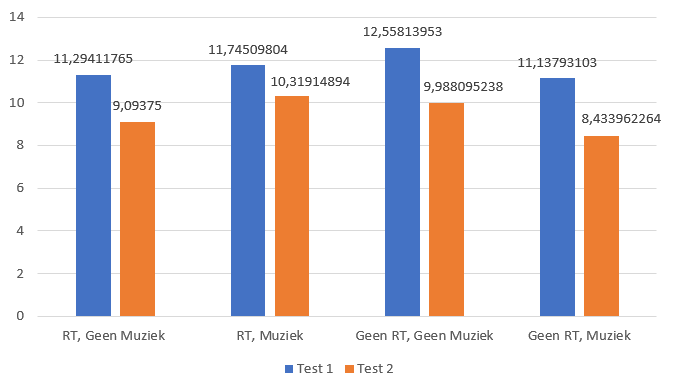
\includegraphics[width=\linewidth]{img/algemeen.png}
		\caption{Globale gemiddelden}
	\end{figure}
	
	\subsection{Uren wiskunde}
	Zoals eerder vermeld zoeken we naar een verband tussen het aantal uren wiskunde verkregen in het middelbaar en het aantal herinnerde feiten op beide retentietesten. Op onderstaande boxplots wordt de spreiding volgens het aantal uren wiskunde geïllustreerd. Er is een duidelijk stijgende trend zichtbaar voor een hoger aantal uren wiskunde waarbij de gemiddelden in de categorieën [3,4] en [5,8] op gelijkaardige hoogte liggen. De resultaten van de 2e testronde liggen lager. Dit komt deels omdat de testpersonen de tekst niet opnieuw mochten lezen maar enkel met zijn herinneringen het invulblad moest indienen. Er zijn opniew gelijkaardige gemiddelden maar in dit geval voor alle geteste categorieën. Merk op, het grootste deel van de groep behaalde een mindere score op de 2e test maar er zijn meer uitschieters.
	
	\begin{figure}[H]
		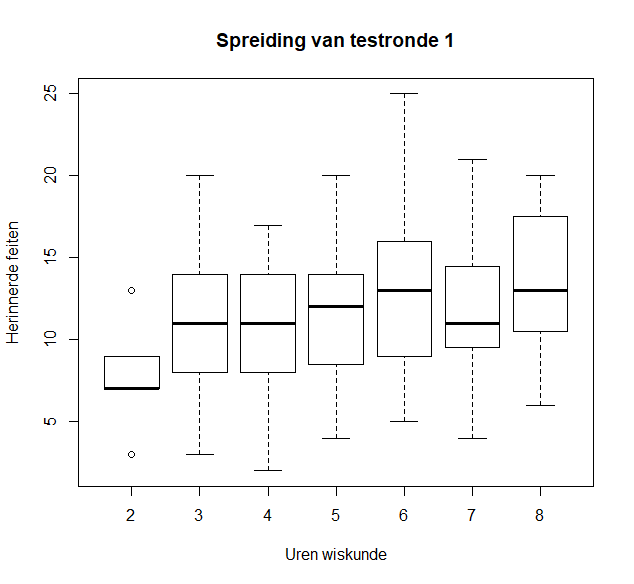
\includegraphics[width=\linewidth]{img/boxplot1.png}
		\caption{Boxplot score 1}
	\end{figure}

	\begin{figure}[H]
		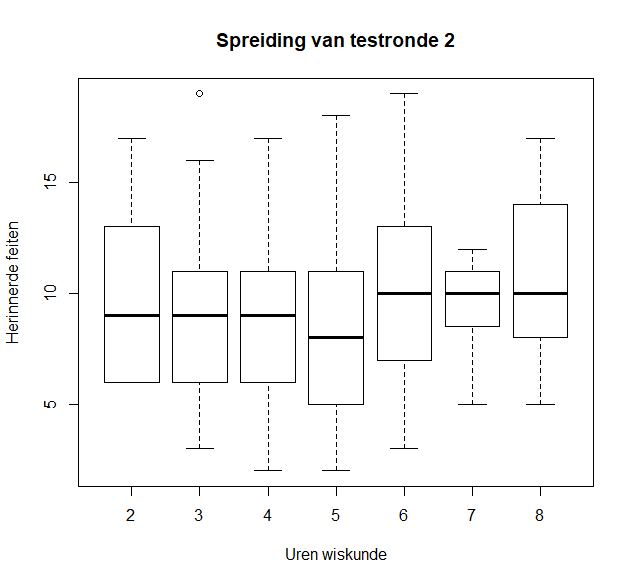
\includegraphics[width=\linewidth]{img/boxplot2.png}
		\caption{Boxplot score 2}
	\end{figure}

	Vervolgens worden de frequenties bekeken, de extreem lage scores vallen direct op en zijn een indicatie naar testpersonen die weinig interesse tonen in het onderzoek (zoals eerder vermeld) en daarom minder hun best hebben gedaan om feiten te herinneren of in de 1e plaats de tekst grondig te analyseren. Hieruit kunt u ook afleiden dat elke categorie genoeg representatief is in het onderzoek.
	
	\begin{figure}[H]
		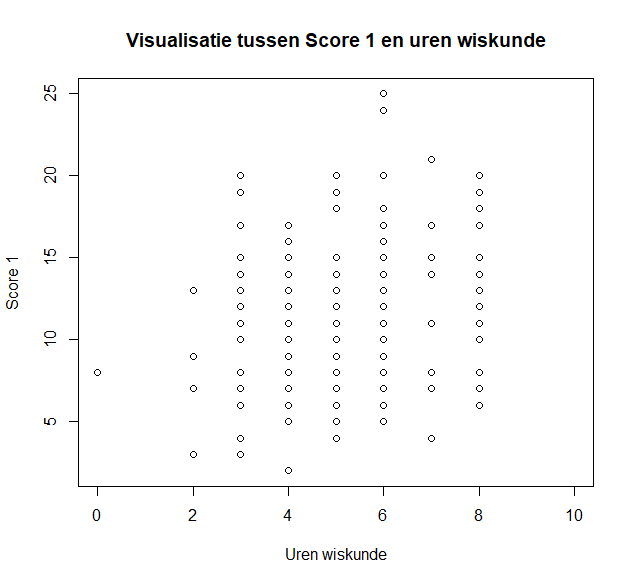
\includegraphics[width=\linewidth]{img/corr1}
		\caption{Frequenties bij score 1 volgens uren wiskunde}
	\end{figure}
	\begin{figure}[H]
		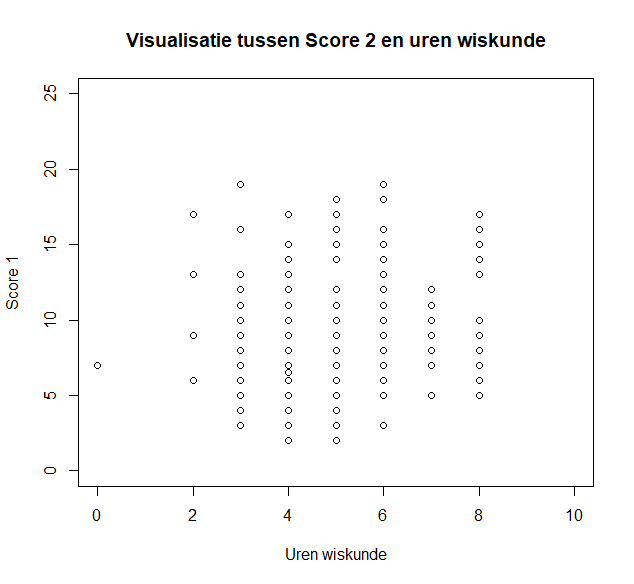
\includegraphics[width=\linewidth]{img/corr2}
		\caption{Frequenties bij score 2 volgens uren wiskunde}
	\end{figure}

	Bovenstaande grafieken tonen de bevindingen van de boxplots op een andere manier aan en zijn dus louter als vervanging die als vermelding gelden voor de frequenties per categorie. Het vertelt dus niks extra over de spreiding van de data.
	We trachten nu om de ligitimiteit van de data te bevestigen. Om een correlatie te vinden kijken we naar het correlatiecoëfficiënt, in dit geval 0,40 (tussen beide scores). Dit nummer geeft het verband weer tussen 2 variabelen. In dit onderzoek zijn 2 verbanden belangrijk (nl. uren wiskunde -> score1/2 en score1 -> score2). Deze data wordt verder gebruikt om een t-test uit te voeren later in het onderzoek en zo onze vermoedens te bevestigen of ontkrachten. Onderstaande correlatiematrix bevat de p-waarden die in dit geval de correlatiecoëfficiënten voorstellen. We kunnen uit deze matrix afleiden dat de coëfficiënten in alle gevallen zeer zwak zijn. Voor de validatie en werking van deze test verwijs ik naar onze Github repository \autocite{Decorte2019}
	\begin{figure}[H]
		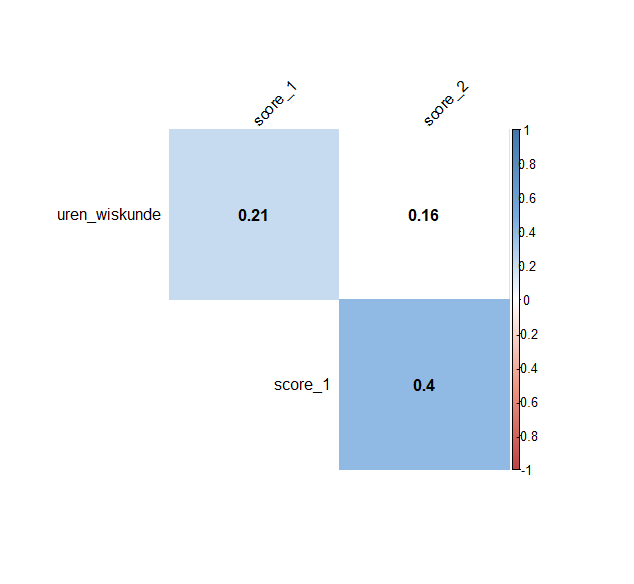
\includegraphics[width=\linewidth]{img/corr.png}
		\caption{Correlatiematrix}
	\end{figure}
	
	Het correlatiediagram geeft duidelijk de spreiding van onze correlatiescore weer tussen het aantal uren wiskunde en de behaalde score. Het is nogmaals duidelijk dat de laag tot extreem lage scores niet in lijn liggen met de verwachte z-waarde. We kunnen zelf beslissen dat deze waarden belachelijk laag liggen tegenover de verwachtingen en dus hoogstwaarschijnelijk te wijten is aan een steekproeffout die tot niet accurate gegevens leidt.
	
	\begin{figure}[H]
		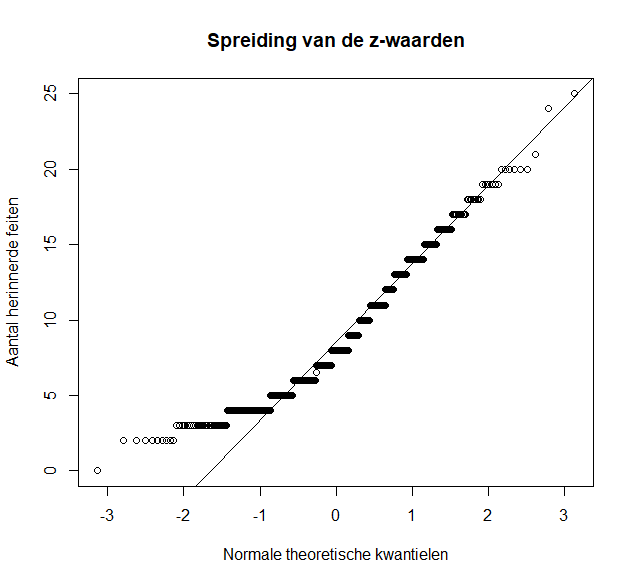
\includegraphics[width=\linewidth]{img/qqplot.png}
		\caption{Q-Q Plot van de dataset idem correlatiediagram}
	\end{figure}

	\subsection{Diploma ouders}
	Voor de 2e hypothese kijken we of studenten met ouders met universitaire achtergrond meer scoorden dan degene zonder. Het valt hier op dat studenten beter scoren indien minimaal één ouder een Bachelor diploma of hoger heeft. In de eerste test zien we voornamelijk een groot verschil in de behaalde scores. Op lange termijn blijk het verschil af te zwakken. Dit komt dus overeen met onze hypothese hierover.
	
	\begin{figure}[H]
		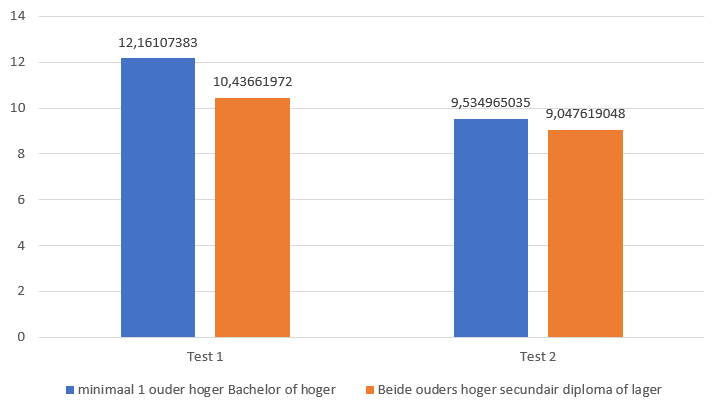
\includegraphics[width=\linewidth]{img/univ.png}
		\caption{Diploma ouders}
	\end{figure}
	
	\subsection{Secundair diploma student}
	De 3e hypothese bekijkt of studenten die ASO deden, beter scoorden dan degene die een andere richting volgden. De resultaten bevestigen ons verwachtingen. We zien dat de ASO groepen zowel in test 1 als test 2 hoger scoorden dan studenten die TSO of BSO richtingen volgden. Hiervoor zien we in beide testen een overduidelijk verschil. Ook na een week scoort ASO duidelijk hoger dan BSO en TSO.
    
	\begin{figure}[H]
        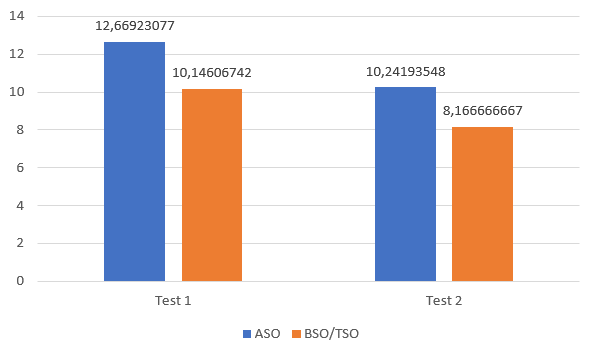
\includegraphics[width=\linewidth]{img/aso.png}
        \caption{aso}
    \end{figure}
	
	
	\subsection{Interesse student}
	De 4e hypothese kijkt of de interesse van de studenten een rol speelt in hun scores. We starten de analyse door een verband te zoeken tussen de scores. Hierbij valt op dat studenten met interesse in het onderwerp beter scoren dan studenten zonder interesse. Bij het uitvoeren van een t-test tussen de studenten die uit een ASO richting komen en diegene uit een andere richting, bekomen we 1.6. Hiermee vinden we de kritieke grenswaarden en het betrouwbaarheidsinterval zonder de standaardafwijking van de steekproef te gebruiken.
    
	
	
	\section{Conclusie}
	Onze verwachtingen waren realtief goed ingeschat. Dankzij dit onderzoek kunnen we besluiten dat studenten die ASO deden in hun hoger secundair deden over het algemeen beter zijn in dingen te onthouden. Dit is duidelijk te merken en beide testen. Eveneens valt er op dat studenten met minstens één ouder die een Bachelor diploma of hoger heeft hoger scoren. Studenten waarvan beide ouders een hoger secundair diploma op lager hebben scoren minder. Op lange termijn (Test 2) zien we wel dat dit verschil veel kleiner wordt. Vervolgens hebben we in dit onderzoek ook kunnen testen of de interesse in een onderwerp je geheugen gaat beïnvloeden. Hiervoor valt ons op dat dit daadwerkelijk een rol speelt. Studenten die geïnteresseerd zijn het onderwerp scoren betere punten dan studenten die dit niet zijn. Ten slotte hebben we uiteraard ook onderzocht of retrieval practice en muziek helpt bij het onthouden van leerstof. Hier kwamen we echter tot een niet verwachte conclusie. Retrieval practice blijkt enkel te helpen indien het gecombineerd wordt met muziek. Bij het gebruik van retieval practice zonder muziek of enkel muziek en geen retieval practice worden de laagste scores behaald. De aller beste optie is raar genoeg zonder muziek en zonder retieval practice.
	
	
	%------------------------------------------------------------------------------
	% Referentielijst
	%------------------------------------------------------------------------------
	% TODO: de gerefereerde werken moeten in BibTeX-bestand ``bibliografie.bib''
	% voorkomen. Gebruik JabRef om je bibliografie bij te houden en vergeet niet
	% om compatibiliteit met Biber/BibLaTeX aan te zetten (File > Switch to
	% BibLaTeX mode)
	
	\phantomsection
	\printbibliography[heading=bibintoc]
	
\end{document}

